% ALICE COMMENTS---
% EMAIL 1:
% General observations- Tritium breeding and power density should also be included in your vocabulary 
% Insert a picture of pebble bed before 1.2 (or move Fig. 1.3 to there)
% Specific sentences: 
% 1) DONE -- Thus to provide designers the ability to optimize breeder volumes for "tritium breeding and subsequent" tritium release,
% 2) DONE -- In this approach, heat transport in pebble beds is often characterized with an effective thermal conductivity, keff,  "and interface heat conductance"
% 3) DONE -- and considerations of "slow moving" inter-porous helium purge gas.
% Question
% Have you showed "and changes to bed stresses and contact-force networks in beds with restructured packing" in the past? 


%%%%%%%%%%%%%%%%%%%%%%%%%%%%%%%%%%%%%%%%%%
\chapter{Introduction} \label{sec:introduction}
%%%%%%%%%%%%%%%%%%%%%%%%%%%%%%%%%%%%%%%%%%
% brief intro of pebble beds
% Sustaining and controlling the fusion of hydrogen reaction can supply the world with a power source which is nearly inexhaustible, relatively free from radiation dangers of traditional fission reactions, and produces no greenhouse gases. Global attention has focused on the most easily-attained fusion reaction,
Fusion research and development activities are proceeding on the expectation that the D-T reaction,
\begin{align}
\ce{D + T -> ^4He + n}+ \SI{17.6}{\mega\electronvolt}
\end{align}
will be used for the first generation fusion reactors based on its energetics and attainability. While deuterium can be readily separated from water and is in great abundance on Earth, tritium is radioactive with $\beta^-$ decay with a half-life of only 12.32 years, rendering it extremely scarce, expensive, and challenging to store and produce. As a consequence, the feasibility of a fusion power reactor hinges on the sustained availability of tritium. Accordingly, fusion reactor designs include a self-sustaining fuel cycle -- breeding tritium in blankets surrounding the fusion core. Breeding blankets will generate tritium \textit{in-situ} from interactions of lithium with neutrons originating either from the fusion reaction directly or neutron multiplication reactions. Relevant lithium reactions are
\begin{align}
\ce{n + ^7Li -> n + ^4He + T}-\SI{2.47}{\mega\electronvolt} \label{eq:Li7T} \\
\ce{n + ^6Li -> ^4He + T} + \SI{4.78}{\mega\electronvolt} \label{eq:Li6T}
\end{align}

%Confinement of fusion is proposed with the complex magnetic fields created in a tokamak device. \Cref{fig:demo} shows an example sketch of a demonstration (DEMO) fusion reactor and the relative location of the breeder blanket modules as they will face the toroidal plasma of a tokamak.
% \begin{figure}[h]
% 	\centering
% 	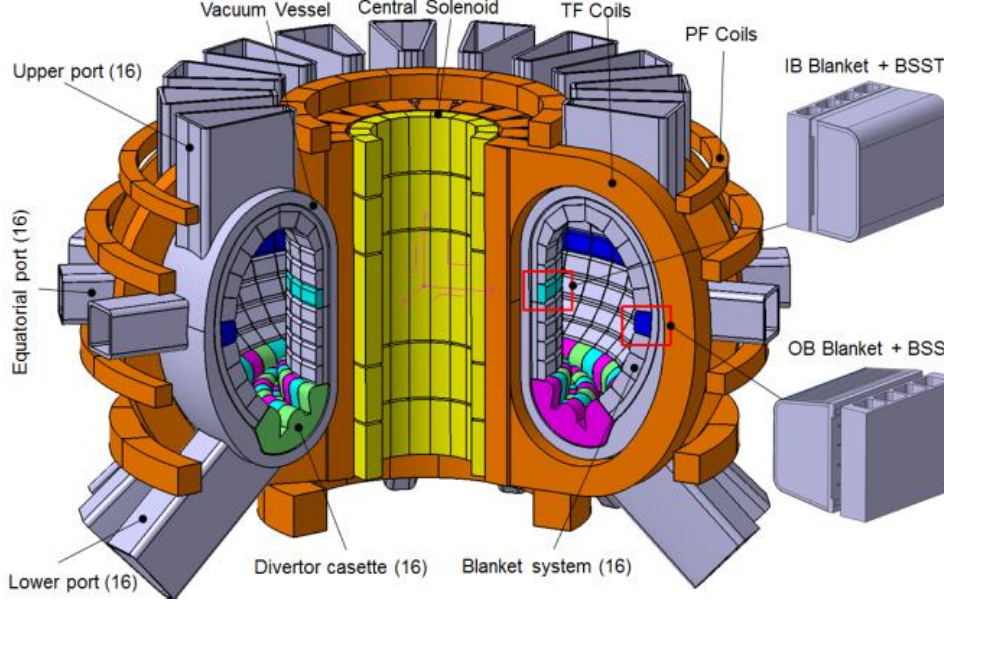
\includegraphics[width=\singleimagewidth]{figures/demo} 
% 	\caption{An example design of a DEMO reactor with solid breeder blankets shown as inboard (IB) and outboard (OB) blanket components.}
% 	\label{fig:demo}
% \end{figure}

Solid lithium materials are potential candidate forms for tritium generation in fusion power plants. Many different potential solid materials have been studied in the past; including inter-metallic compounds (\textit{e.g.} \ce{Li7Pb2}), lithium oxide (\lio), and ternary oxides (\textit{e.g.} \lis, \lit, \lial, \liz, \textit{etc.}). Solid breeder materials offer a number of potential safety advantages including relatively low tritium mobility and low stored chemical energy.

In the years since the solid breeder concept inception, the fusion community has come to recognize that lithium-based oxides (including ceramic oxides) are the most promising tritium-breeding materials for fusion reactor solid breeder blankets. This conclusion is based on oxides having many desirable characteristics, such as: 
\begin{itemize}
\item{high Li density}
\item{high melting temperature}
\item good tritium release (sufficiently high T release rates, low solubility, and open porosity for purging T)
\item good thermophysical and thermomechanical characteristics
\item ability to withstand the rigors of long-term irradiation at high temperature and under large temperature gradients
\item{desirable neutronics and irradiation characteristics (no bad transmutation nuclides)}
\item{chemical stability \& compatibility with structural material at operating temperatures (in particular thermal stability and chemical inertness are attractive from a safety point of view)}
\end{itemize}

Calculations of other candidate materials indicate that inter-metallic compounds have unacceptable operating temperatures (exceedingly narrow temperature windows) and are unattractive for in-situ tritium recovery. In addition, the compounds of \ce{Li7Pb2} and \ce{Li62Pb38} were shown to vigorously react with water and do not offer significant safety advantages compared to liquid breeders.\cite{Clemmer1980,Abdou1975c} And a major emphasis of blanket/breeder design is placed on safety and environmental acceptability, with primary goals of low tritium inventory in the blanket and minimal long-lived activation products. Therefore this research is focused entirely on discussion of lithium ceramics and modeling thereof.

Reference solid breeder engineering designs have converged toward liquid-cooled pebble beds of lithium ceramics.  Pebble bed designs incorporate packed ceramic pebbles (spherical particles) that are filled into containment structures of a reduced-activation ferritic steel. In a typical solid breeder module, the breeding volume is subdivided into several alternating layers of neutron multiplication material (generally beryllium) and tritium breeding material. The layers are separated by plates with internal channels for flowing liquid coolant. Coolants are typically a high pressure helium, though some designs call for pressurized water, in spite of the dangers of the highly exothermic reaction of lithium with oxygen from water vapor in the case of coolant leak. The coolant, heated as it passes through tritium breeding modules, proceeds into a standard electricity production cycle. After tritium is generated inside the ceramic, the bred hydrogen isotope is ultimately picked up by a low-pressure, slow-moving purge gas (primarily helium) and extracted in a closed loop for fuel. 

Pebble bed forms of tritium breeding volumes have several advantages which include: ease of assembly of granular materials into complex geometries; bred tritium can be readily removed \textit{via} the helium purge gas through interstitial porous networks; ceramic material is unaffected by the large magnetic fields confining the plasma, and temperature gradients across any single pebble are small enough to avoid damage from thermal stress. A sketch of a generic ceramic pebble bed volume depicting all the features described above is given in \Cref{fig:solid-breeder-sketch}.

\begin{figure}[ht]
	\centering
	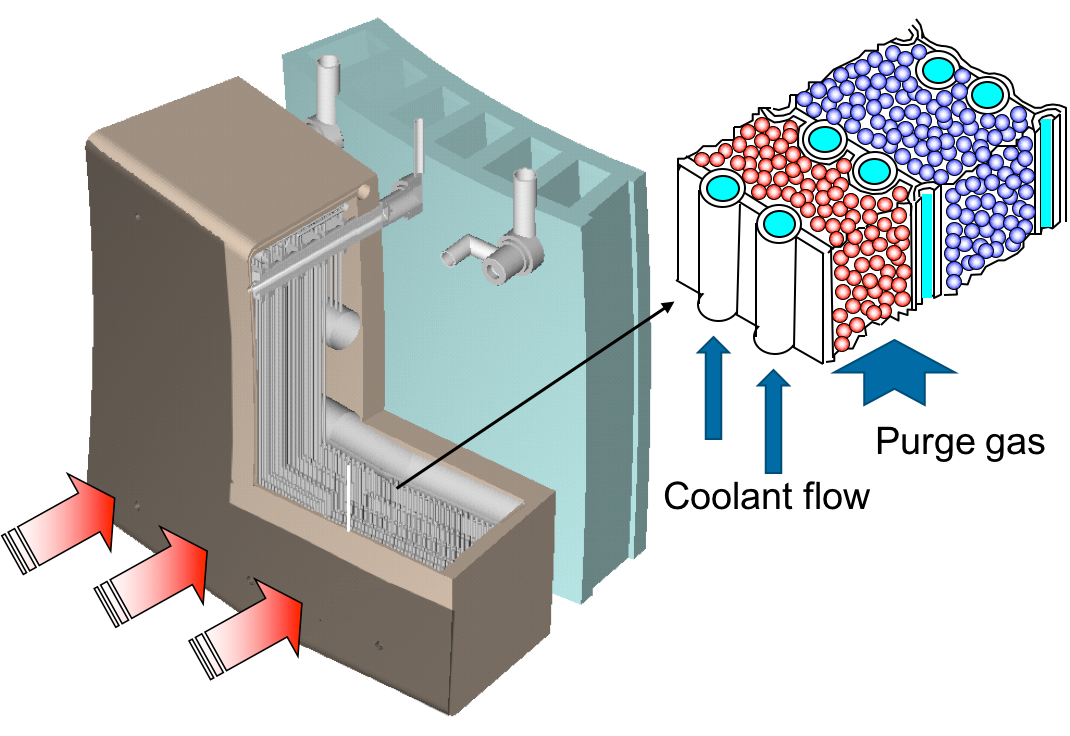
\includegraphics[width=\singleimagewidth]{figures/JP-solid-breeder-sketch} 
	\caption{Example sketch of a typical solid breeder design (from an early Japanese ITER sketch). Showing: heat flux on first wall, layered solid breeder (red pebbles) and neutron multiplier (blue pebbles), separated by a structure with internally flowing coolant, and purge gas flowing through tritium breeding zone.}
	\label{fig:solid-breeder-sketch}
\end{figure}


\section{Solid Breeder Thermal Management and Imposed Temperature Window}

The feasibility of the solid breeder concept is based on the capability of tritium to readily transport from the solid ceramic into the purge gas. Tritium release, itself, is a function of grain size, microsctructure, and open/closed porosity. To understand the capability of tritium removal, five mechanistic steps are identified for bred tritium to be recovered (visualized in \Cref{fig:mechanisms_tritium_transport}). The steps follow as\cite{Clemmer1980}
\begin{enumerate}
\item bulk diffusion,
\item grain boundary migration,
\item desorption of tritium (T$_2$O),
\item percolation of tritium through pores internal to the solid ceramic toward the flowing purge gas,
\item convective mass transfer out of the blanket via purge channels.
\end{enumerate}

\begin{figure}[ht]
	\centering
	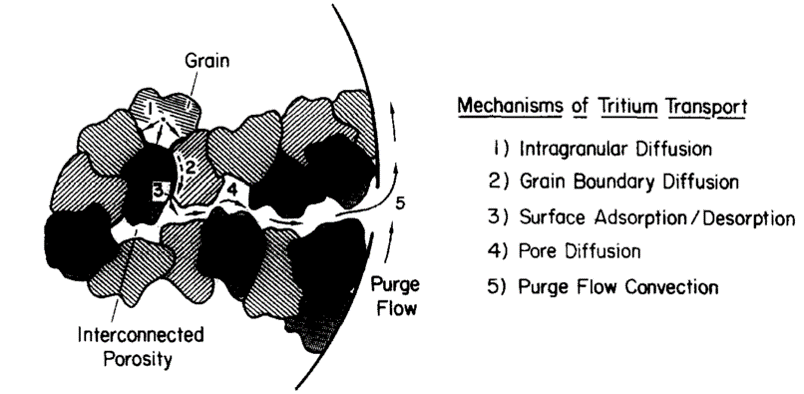
\includegraphics[width=0.75\textwidth]{figures/mechanisms_tritium_transport} 
	\caption{Mechanistic steps of tritium transport through ceramic materials into the purge gas for removal. Image reproduced from Ref.\cite{hastings1989fabrication}}
	\label{fig:mechanisms_tritium_transport}
\end{figure}

Bulk diffusion of tritium is considered to be a significant contributor to tritium inventory. For spherical particles of radius $r_p$, assuming zero surface concentration, the tritium inventory $T$ is given by 
\begin{equation}\label{eq:inventory-diff}
T = \frac{1}{15}\dot{T}\frac{r_p^2}{D}
\end{equation}
where $\dot{T}$ is the tritium generation rate and $D$ is diffusivity of tritium in the ceramic. It is significant to note that the tritium inventory is a function of the square of the particle size. Thus it is clear that: (i) small grain sizes are required for minimum tritium inventory and (ii) grains should not significantly grow during the lifetime of a reactor blanket. Diffusivity values of tritium in ceramics are extremely scarce and with much uncertainty. Kinetic experiments of post-irradiation tritium release from several candidate breeders have been performed. The kinetics in the experiments are non-steady-state and the diffusivity is given by 
\begin{equation}\label{eq:exp-diff}
D = 0.16 \frac{r_p^2}{\tau}
\end{equation}
where $\tau$ is the mean residence time, defined as the time required to extract 87.4\% of the tritium. Combining \Cref{eq:inventory-diff} and \Cref{eq:exp-diff} eliminates diffusivity and radius (with large variation between particles and grains), yielding:
\begin{equation}
T = 0.42 \dot{T}\tau
\end{equation}

We can then estimate the diffusive inventory in a blanket based on the readily-measured residence time, $\tau$. It must be kept in mind that the particular micro-structure of the ceramics measured in kinetic experiments must correspond to the micro-structure of the material in the blanket in order for the diffusivity predictions to hold. In other words, residence times of \SI{1}{\milli\meter} \lit~with average grain sizes of $\mu = \SI{1}{\micro\meter}$ are utterly inappropriate to calculate tritium diffusion in \SI{0.5}{\milli\meter} pebbles of \lis~with average grain sizes of $\mu = \SI{5}{\micro\meter}$, for example.

The tritium generation rate, $\dot{T}$ is a function of the fusion reactor power output and blanket design. Residence times have been measured to be temperature dependent which is consistent with diffusion-controlled processes. Therefore, based on the present model, the range of operating limitations are defined on the low end where bulk diffusion is the rate-limiting step. A minimum temperature is defined as the temperature at which the tritium inventory exceeds \SI{1}{\kilo\gram\per\giga\watt}. The minimum temperatures for many candidate materials are shown (with slight variation between sources) in \Cref{fig:Tmin}. Minimum temperatures generally range from 300 up to \SI{400}{\celsius}.

\begin{figure}[ht]
	\centering
	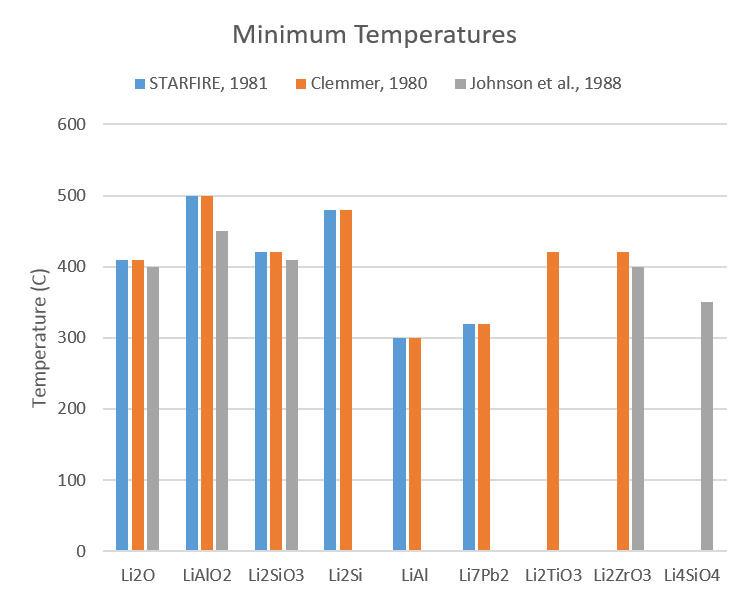
\includegraphics[width=0.9\textwidth]{figures/Tmin} 
	\caption{Minimum temperatures for various candidate materials (compiled from various sources) based on rate-limiting diffusion processes. STARFIRE data from Ref.\cite{Johnson1981}, Clemmer from Ref.\cite{Clemmer1980}, Johnson\etal~from Ref.\cite{Johnson1988}}
	\label{fig:Tmin}
\end{figure}

As we saw from \Cref{eq:inventory-diff}, tritium inventory goes with the square of grain size and thus another operating limit on temperature arises. An upper limit of temperature is based on restructuring or grain growth in ceramics which can greatly affect the diffusive inventories. When ceramic materials are heated above their sintering temperature, generally in excess of $0.8 T_\text{melt}$ (in absolute temperature), grains will grow. 

Moreover, when lithium depletion (or lithium burn-up) occurs to a significant extent (around 5\%), the resultant nonstoichiometry in ternary oxides could establish, rather than single-phase conditions. For example, under irradiation and lithium burn-up, \lis~ceramics would develop an excess of silica and the melting point of \SI{1300}{\celsius} would drop to a eutectic temperature of \SI{1024}{\celsius}. Such a reduction in melt temperature would have significant impact on sintering and tritium inventory in the solid breeders.\cite{Johnson1981} Therefore, neutron radiation influences are generally expected to lower the maximum operational temperature to $0.6 T_\text{melt}$.\cite{Johnson1981} Candidate materials are compared in \Cref{fig:Tmax}. In general, acceptable candidate materials have their maximum temperature between 750 and \SI{900}{\celsius}. 

\begin{figure}[ht]
	\centering
	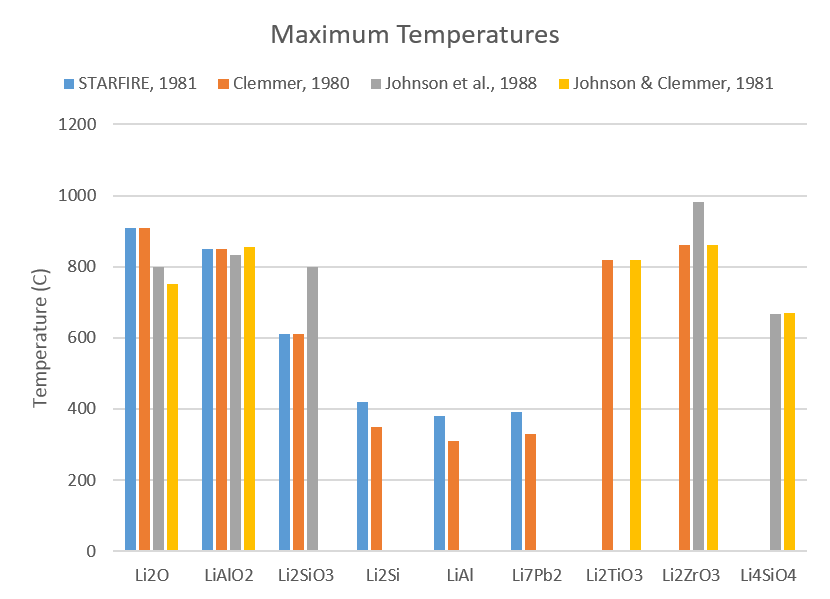
\includegraphics[width=0.9\textwidth]{figures/Tmax} 
	\caption{Maximum temperatures for various candidate materials (compiled from various sources) based on irradiated sintering temperatures ($0.6T_\text{melt}$). STARFIRE data from Ref.\cite{Johnson1981}, Clemmer from Ref.\cite{Clemmer1980}, Johnson\etal~from Ref.\cite{Johnson1988}}
	\label{fig:Tmax}
\end{figure}

As a consequence of the tritium inventory of solid breeder material, we are faced with a relatively narrow operational temperature to which solid breeder designers must adhere, roughly between 350 and \SI{800}{\celsius}. Thus to provide designers the ability to optimize breeder volumes for tritium breeding and subsequent tritium release, we must understand the important physics and phenomena dictating thermophysical properties and thermomechanical responses of pebble beds during operation in a fusion reactor. 


% High energy (14 MeV) neutrons are ejected from the deuterium-tritium reaction, as described by \Cref{eq:dt-reaction}
% \begin{align}
%     \mathrm{D} + \mathrm{T}&\xrightarrow{}\ ^4\mathrm{He}+\mathrm{n}+17.58\ \text{MeV} \label{eq:dt-reaction}
% \end{align}
% thus t

Tritium breeding blankets will experience high volumetric heating as deposited by high-energy neutrons that are carrying away approximately 80\% of the fusion reaction energy in addition to heating from secondary $\gamma$ rays. Heat deposited in breeders must be transported through pebble bed regions into the walls of containing structures, then ultimately into the coolant gas. Heat deposited into pebble beds will transfer \textit{via} inter-particle contact conduction, inter-particle radiation, and convection with the helium purge gas. At the interface with the structural material, similar modes of heat transfer are present: particle-wall contact conduction, particle-wall radiation, and communication \textit{via} helium purge gas convection. 

There exists a coupling between mechanical forces acting upon beds and their heat transport capabilities, thus we must understand packing structures in order to understand heat transfer. The structure of packed beds can be considered as a metastable configuration that will last indefinitely unless acted upon by an external perturbation such as vibration or compressive pressure.\cite{Jaeger1996} The ability of a metastable configuration to resist perturbations can, in some way, be quantified by the initial packing fraction. For more compliant beds (lower packing fractions), stresses from thermal expansion can cause significant rearrangement of the packing structure which is not recoverable after stress removal. This phenomena has been observed in numerous experiments as so-called plastic rearrangement of pebble beds.\cite{Reimann:2002kl,Reimann:2000tw,Zhang2015} Plasticity of beds may have significant consequences for the ability of the pebble bed to maintain contact with the containing structure and routes for heat out of the bed due to gap formation between pebble volumes and coolant walls. 

Moreover, as pebbles heat under nuclear loads, thermal expansion of pebbles in the packed volume will be contained by cooler structural material. Confined expansion will give rise to increased contact pressure between pebbles. Increased pressure between pebbles can cause, among other effects, brittle pebbles to fragment. Therefore, some amount of restructuring of pebble beds (and internal contact force networks) are also likely to occur from crushing/cracking of individual pebbles, or the effects of inter-pebble sintering and creep arising from the high-temperature, high-stress environment in a solid breeder unit. Contact conduction in beds, intimately linked to the packing structure, will be impacted during operation of ceramic pebble beds in fusion reactors.

Because tritium inventory requirements impose a relatively narrow operational temperature window on lithium ceramic pebble beds, and given the high power densities in fusion power reactors, it is necessary to have accurate knowledge of ceramic pebble bed thermomechanical behavior and comprehensive characterization; reliable models of heat transfer in solid breeders are critical for solid breeder designs. In addition, due to the complicated nature of granular materials, heat transfer in these solid breeder volumes remains transient during fusion operation. Concurrently, interaction of the slow-moving purge gas with tightly packed pebble beds is an additional route of heat transfer that must be understood. Thus, heat transfer in pebble beds is quite different from standard solid materials and requires specialized modeling of the synergistic physics. Knowledge and characterization of thermal transport must anticipate changes to the heat transfer capabilities and predict temperature profiles for pebble bed packing structures that will emerge after initially-packed pebble beds react to prolonged exposure to fusion reactor environments.


\section{Objectives of this Study}\label{sec:intro-scope-of-work}
The goal of this work is to develop more comprehensive and accurate models for predicting temperature distributions in ceramic breeder pebble beds, accounting for many important phenomena including pebble crushing and fragmentation, dynamic analysis of packing restructuring, and considerations of slow moving inter-porous helium purge gas. 

Modeling will be done with discrete element method (DEM) models coupled to computational fluid dynamics (CFD) and lattice-Boltzmann method (LBM) descriptions of fluid flow. In particular detailed relationships between topological changes to packing structures, arising from fragmented pebbles, and the resulting changes to heat transfer in packed beds will be considered. For the first time, attention will be given to nuclear heating of pebble fragments as they redistribute through pebble beds and come to rest without strong mechanical contact (and therefore contact conductance) to neighboring pebbles. This includes analyzing changes to temperature distributions in pebble beds with different models of pebble damage, analyzing the impact of helium flow on temperatures in beds with fragmented pebbles, and changes to bed stresses and contact forces in beds with restructured packing. Furthermore, changes to effective thermal conductivity in packed beds with simulated reduction in solid conductivity due to irradiation damage of ceramic pebbles will be considered. 

While it is the aim of this study to provide fusion blanket designers with the most complete models possible for predictive capabilities of temperature distributions in solid breeders such that operability margins to tolerate irradiation damage or crushed pebbles may be expanded, it is understood that the models developed here will not, on their own, provide a total description of physics governing heat transfer in solid breeder pebble beds during operation. As will be pointed out later in this thesis, effects of radiation, fluid slip, sintering, and creep are all phenomena that can play a role in pebble bed heat transfer but are beyond the scope of the current work. Therefore, it is also the goal of this thesis to develop modeling tools in a modular method on well-supported, open-source frameworks which will facilitate adoption of this code and permit future expansion to conjoin with modules describing other physics. In this way, the code developed for thesis can be adopted by the community at large and expanded upon in future research.